\documentclass[a4paper,10pt]{report}\input{../0.Préambule/Préambule_cours_prof}\begin{document}

\pagestyle{empty}
\newpage
\noindent NOM, Prénom et classe : \dotfill

\section*{Nombres relatifs}
\addcontentsline{toc}{section}{Nombres rationnels et pourcentages}

\noindent \textit{Il sera tenu compte dans la notation de la propreté ainsi que de la justification apportée à chacune des réponses.}

\noindent \textit{Le barème est donné à titre indicatif. Il pourra être modifié ultérieurement.}

\noindent \textit{L'usage de la calculatrice est \textbf{interdite}.} \hfill \textit{Durée : 55 minutes}

\medskip
\paragraph{Exercice 1}: \hfill \textbf{3 points}

Complète avec le mot qui convient : 
\begin{center}
 \og positif \fg{} \quad \og négatif \fg{} \quad \og plus \fg{} \quad \og relatifs \fg{} \quad \og opposé \fg{} \quad\og moins \fg{}
\end{center}

\begin{enumerate}
\item $-3$; $+5$; $-9,3$; $100,7$ et $0$ sont des nombres \dotfill \medskip
\item Le nombres $+5$ est un nombre \dotfill \medskip
\item Il peut aussi s'écrire sans le signe \dotfill \medskip
\item Le nombre $-5$ est un nombre \dotfill \medskip
\item On ne peut pas supprimer le signe \dotfill \medskip
\item $-2,7$ est  \dotfill de $+2,7$.
\end{enumerate}

\medskip
\paragraph{Exercice 2}: \hfill \textbf{3 points}

\begin{enumerate}
\item Sur la droite gradué, d'unité de longueur le centimètre, place les points $A(+0,8)$, $B(-2,3)$, $C(+3,5)$, $D(+5,4)$ et $E(-1,6)$.

\begin{center}
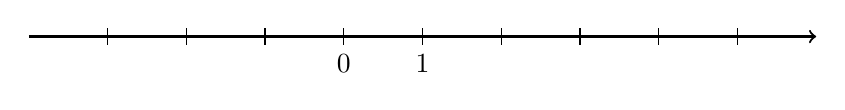
\begin{tikzpicture}[x=1cm]  
\draw[thick,->] (-4,0) -- (6,0);
\foreach \x in {0,1}
\draw[shift={(\x,0)},color=black] (0pt,3pt) -- (0pt,-3pt) node [below] {\x};
\foreach \x in {,-3,-2,-1,2,3,4,5}	
\draw[shift={(\x,0)},color=black] (0pt,3pt) -- (0pt,-3pt) ;
\end{tikzpicture}
\end{center}

\vspace{-5mm}
\item En examinant la position des points $A$, $B$, $C$, $D$ et $E$ sur cette droite gradué, range dans l'ordre décroissant : $+0,8$, $-2,3$, $+3,5$, $+5,4$ et $-1,6$.
\end{enumerate}

\noindent\grandscarreaux{\linewidth}{1.6cm}

\medskip
\paragraph{Exercice 3}: \hfill \textbf{3 points}

\begin{minipage}{9cm}
\begin{enumerate}
\item Donne l'abscisse du point $A$

\noindent\grandscarreaux{\linewidth}{0.8cm}

\item Donne l'ordonnée du point $A$.

\noindent\grandscarreaux{\linewidth}{0.8cm}
\item Quelles sont les coordonnées du point $B$ ?

\noindent\grandscarreaux{\linewidth}{0.8cm}
\item Place dans le repère ci contre le point $C$ d'abscisse $-2$ et d'ordonnée $-1$.
\item Place le point $D(1;-1)$.
\end{enumerate}
\end{minipage}
\begin{minipage}{8cm}
\begin{center}
\begin{tikzpicture}[line cap=round,line join=round,>=triangle 45,x=1.0cm,y=1.0cm,scale=0.7]
\begin{axis}[x=1.0cm,y=1.0cm,axis lines=middle,ymajorgrids=true,xmajorgrids=true,
xmin=-3.3,xmax=4.3,ymin=-2.3,ymax=5.3,xtick={-3.0,-2.0,...,3.0,4.0},ytick={-2.0,-1.0,...,5.0},]
\clip(-3.3,-2.3) rectangle (4.3,5.3);
\draw [line width=1.2pt,dash pattern=on 4pt off 4pt] (-1.,2.)-- (-1.,0.);
\draw [line width=1.2pt,dash pattern=on 4pt off 4pt] (-1.,2.)-- (0.,2.);
\draw [line width=1.2pt,dash pattern=on 4pt off 4pt] (3.,4.)-- (0.,4.);
\draw [line width=1.2pt,dash pattern=on 4pt off 4pt] (3.,4.)-- (3.,0.);
\begin{scriptsize}
\draw [color=blue] (-1.,2.)-- ++(-3.5pt,0 pt) -- ++(7.0pt,0 pt) ++(-3.5pt,-3.5pt) -- ++(0 pt,7.0pt);
\draw[color=blue] (-0.86,2.45) node {\large{$A$}};
\draw [color=blue] (3.,4.)-- ++(-3.5pt,0 pt) -- ++(7.0pt,0 pt) ++(-3.5pt,-3.5pt) -- ++(0 pt,7.0pt);
\draw[color=blue] (3.14,4.45) node {\large{$B$}};
\end{scriptsize}
\end{axis}
\end{tikzpicture}
\end{center}
\end{minipage}

\medskip
\paragraph{Exercice 4}: \hfill \textbf{4 points}

\noindent Complète par $<$, $>$ ou $=$
\begin{enumerate}
\renewcommand{\arraystretch}{1.5}
\begin{tabularx}{\linewidth}{*{4}{>{\arraybackslash}X}}
\item $10 ~\dots ~ \dots ~ +3$&
%\item $-5 ~\dots ~ \dots ~ -5,0$&
\item $-8 ~\dots ~ \dots ~ 0$&
\item $0 ~\dots ~ \dots ~ -4$&
\item $+3 ~\dots ~ \dots ~ 0$\\
\item $3,14 ~\dots ~ \dots ~ -1,732$&
\item $-9,27 ~\dots ~ \dots ~ -9,272$&
\item $+8,64 ~\dots ~ \dots ~ -8,64$&
%\item $-19,2 ~\dots ~ \dots ~ +9,2$&
\item $-14,39 ~\dots ~ \dots ~ +14,4$\\
\end{tabularx}
\end{enumerate}



\medskip
\paragraph{Exercice 5}: \hfill \textbf{7 points}

Louane souhaite utiliser le système de géolocalisation de son téléphone pour se rendre chez une amie. Pour cela, le téléphone doit d'abord trouver son positionnement.

\medskip
\noindent Quelles sont les coordonnées du point ou se trouve Louane actuellement ?

\medskip
\noindent \textit{Toute piste de recherche même infructueuse sera pris en compte}

\begin{doc}[La géolocalisation GSM]
\begin{enumerate}
\item[•] Le principe de la géolocalisation par téléphone mobile (géolocalisation GSM) repose sur la mesure de la distance entre le téléphone et les antennes du réseau de téléphonie mobile.
\item[•]Le positionnement d'un point est déterminé en croisant les données de plusieurs antennes.
\end{enumerate}
\end{doc}

\begin{doc}[Les relevés]
\renewcommand{\arraystretch}{1}
\begin{tabularx}{\linewidth}{|p{4.5cm}|*{4}{>{\centering \arraybackslash}X|}}
\hline
\rowcolor{doc!10}Antenne & $A$ & $B$ & $C$ & $D$ \\\hline
\cellcolor{doc!10}{Coordonnées de l'antenne (dans un repère d'unité 10km)} & $(30;50)$ & $(70;20)$ & $(0;-20)$ & $(80;140)$ \\\hline
\cellcolor{doc!10}{Distance avec Louane} & $30$km & $40$km & $50$km & $130$km \\
\cellcolor{doc!10}{(donnée par le téléphone)} & & & & \\\hline
\end{tabularx}
\end{doc}

\noindent \begin{minipage}{9cm}
\begin{doc}[Début de la recherche de position]
\begin{tikzpicture}[line cap=round,line join=round,>=triangle 45,x=0.05cm,y=0.05cm,scale=1.2]
\begin{axis}[x=0.05cm,y=0.05cm,axis lines=middle,ymajorgrids=true,xmajorgrids=true,
xmin=-41.0,xmax=91.0,ymin=-25.0,ymax=145.0,xtick={-60.0,-50.0,...,90.0},ytick={-20.0,-10.0,...,140.0},]
\clip(-41.,-25.) rectangle (91.,145.);
\draw [line width=1pt] (30.,50.) circle (1.5cm);
%\draw (12.994331527247493,56.92897450966192) node[anchor=north west] {EA = 30};
%\draw [line width=1pt] (70.,20.) circle (2.cm);
%\draw [line width=1pt] (0.,-20.) circle (2.5cm);
%\draw [line width=1pt] (80.,140.) circle (6.5cm);
\begin{scriptsize}
\draw [fill=blue] (30.,50.) circle (1.5pt);
\draw[color=blue] (33,55) node {\large{$A$}};
\draw [fill=blue] (70.,20.) circle (1.5pt);
\draw[color=blue] (73,25) node {\large{$B$}};
%\draw [fill=blue] (0.,-20.) circle (2.5pt);
%\draw[color=blue] (1.325767113118657,-16.485743262565517) node {$C$};
%\draw [fill=blue] (80.,140.) circle (2.5pt);
%\draw[color=blue] (81.44990942346999,143.56806528456875) node {$D$};
\end{scriptsize}
\end{axis}
\end{tikzpicture}
\end{doc}
\end{minipage}
\hspace{5mm}
\begin{minipage}{7.2cm}
\noindent\grandscarreaux{\linewidth}{11.2cm}
\end{minipage}

\end{document}